WeChat Android is compiled and run on Android platform. This section presents the overview 
of Android OS architecture and Android application. 
\subsection{Android OS}
Android Operation System (OS) is a open-sourced Linux based software stack as represented in 
Figure~\ref{fig:androw_framework}. Majority Android phone manufacture customized their own 
Android OS such as adding or removing a service to Android framework or use different version of 
underlying Linux kernel.

Each Android app is complied into dex-code and installed in the Android OS. When a app is 
launched, it runs within a individual sandbox, namely Dalvik Virtual Machine (VM), from other 
running apps. At run-time, Dalvik Virtual Machine translate the dex-code into machine code and 
execute it. Android 4.4 version introduces an experimental Android Run-time (ART) feature that 
allows device to translate the app's whole dex-code into machine during installation to enable 
faster execution. 

Android apps use Android API to request Android framework services such as make 
phone calls and read photograph. Developers are also allowed to write their application libraries 
in C/C++ as Native libraries and call them through Java Native Interface (JNI). This allows them 
to have low-level access to the system resources (e.g., memory, I/O, and etc) and reuse 
codebase that is implemented in C/C++.  

\begin{figure}
	\centering
	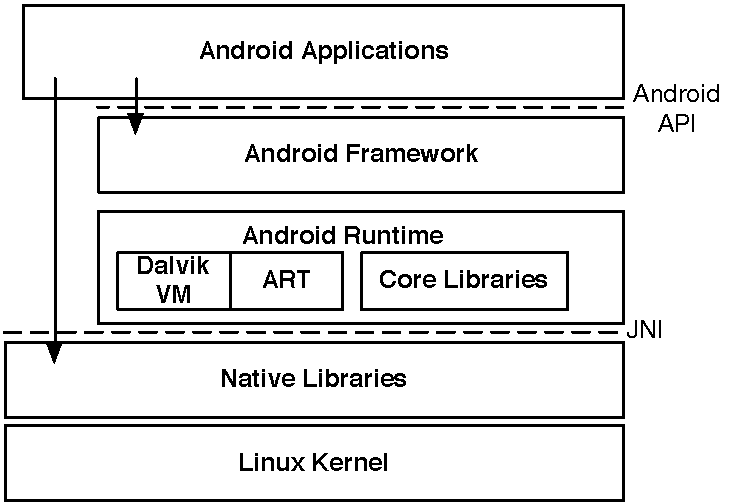
\includegraphics[height=2in, width=3.2in]{android_framework.pdf}
	\caption{Android OS Architecture}
	\label{fig:androw_framework}
\end{figure}

\subsection{Android Application}
Android app consists of four types of components:

\begin{itemize}
	\item \textit{Activity} Each activity is associated with a GUI screen that contains a set of layouts 
	to carry out certain tasks. Each layout defines a set of GUI widgets (e.g., Button, 
	EditText and ImageView) and their orientation. Each widget can be assigned with callback 
	functions such that if delegated event (e.g., click) is triggered, the callback function will be 
	executed. 
	\item \textit{Intents and intent filters} Intents is a messaging object that allows components to 
	communicate with each other. Intent filters only allows designated intent type to be received 
	and processed by the component.  Introduce explicit intent and implicit intent?
	\item \textit{Service} Service is a component that can perform long-term running tasks in the 
	background without GUI screen.
	\item \textit{Content provider} Content provider gives the capability to manage structured set 
	of data such as read contact information. 
	
\end{itemize}